\documentclass{standalone}
\usepackage{pgfplots}
\usepackage{xcolor}
\begin{document}
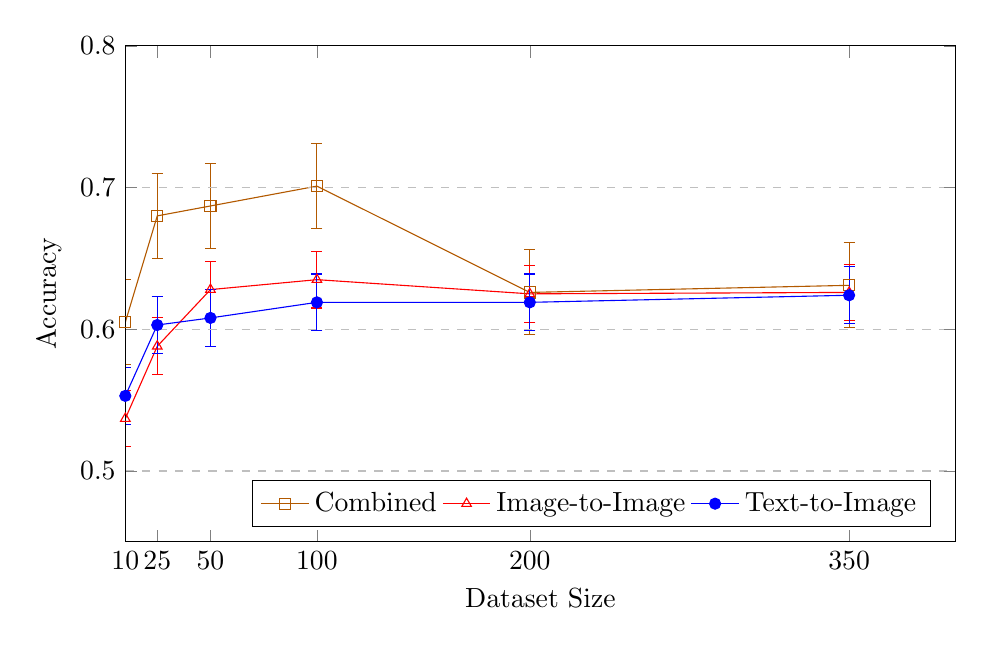
\begin{tikzpicture}
\begin{axis}[
    width=\linewidth,
    height=0.65*\linewidth,
    xlabel={Dataset Size},
    ylabel={Accuracy},
    xmin=10, xmax=400,
    ymin=0.45, ymax=0.8,
    xtick={10,25,50,100,200,350},
    ytick={0.5,0.6,...,0.8},
    legend style={at={(0.97,0.03)},anchor=south east,legend cell align=left},
    axis on top,
    tick label style={/pgf/number format/fixed},
    %ybar,
    ymajorgrids=true,
    grid style=dashed,
    legend columns=-1,
]
\addplot[
    color=orange!70!black,
    mark=square,
    error bars/.cd,
    y dir=both,
    y explicit,
]
coordinates{(10,0.605) +- (0, 0.03)(25,0.680) +- (0, 0.03)(50,0.687) +- (0, 0.03)(100,0.701) +- (0, 0.03)(200,0.626) +- (0, 0.03)(350,0.631) +- (0, 0.03)};
\addplot[
    color=red,
    mark=triangle,
    error bars/.cd,
    y dir=both,
    y explicit,
]
coordinates{(10,0.537) +- (0, 0.02)(25,0.588) +- (0, 0.02)(50,0.628) +- (0, 0.02)(100,0.635) +- (0, 0.02)(200,0.625) +- (0, 0.02)(350,0.626) +- (0, 0.02)};
\addplot[
    color=blue,
    mark=*,
    error bars/.cd,
    y dir=both,
    y explicit,
]
coordinates{(10,0.553) +- (0, 0.02)(25,0.603) +- (0, 0.02)(50,0.608) +- (0, 0.02)(100,0.619) +- (0, 0.02)(200,0.619) +- (0, 0.02)(350,0.624) +- (0, 0.02)};
\legend{Combined, Image-to-Image, Text-to-Image}
\end{axis}
\end{tikzpicture}
\end{document}